% Options for packages loaded elsewhere
\PassOptionsToPackage{unicode}{hyperref}
\PassOptionsToPackage{hyphens}{url}
\PassOptionsToPackage{dvipsnames,svgnames,x11names}{xcolor}
%
\documentclass[
]{agujournal2019}

\usepackage{amsmath,amssymb}
\usepackage{iftex}
\ifPDFTeX
  \usepackage[T1]{fontenc}
  \usepackage[utf8]{inputenc}
  \usepackage{textcomp} % provide euro and other symbols
\else % if luatex or xetex
  \usepackage{unicode-math}
  \defaultfontfeatures{Scale=MatchLowercase}
  \defaultfontfeatures[\rmfamily]{Ligatures=TeX,Scale=1}
\fi
\usepackage{lmodern}
\ifPDFTeX\else  
    % xetex/luatex font selection
\fi
% Use upquote if available, for straight quotes in verbatim environments
\IfFileExists{upquote.sty}{\usepackage{upquote}}{}
\IfFileExists{microtype.sty}{% use microtype if available
  \usepackage[]{microtype}
  \UseMicrotypeSet[protrusion]{basicmath} % disable protrusion for tt fonts
}{}
\makeatletter
\@ifundefined{KOMAClassName}{% if non-KOMA class
  \IfFileExists{parskip.sty}{%
    \usepackage{parskip}
  }{% else
    \setlength{\parindent}{0pt}
    \setlength{\parskip}{6pt plus 2pt minus 1pt}}
}{% if KOMA class
  \KOMAoptions{parskip=half}}
\makeatother
\usepackage{xcolor}
\setlength{\emergencystretch}{3em} % prevent overfull lines
\setcounter{secnumdepth}{5}
% Make \paragraph and \subparagraph free-standing
\makeatletter
\ifx\paragraph\undefined\else
  \let\oldparagraph\paragraph
  \renewcommand{\paragraph}{
    \@ifstar
      \xxxParagraphStar
      \xxxParagraphNoStar
  }
  \newcommand{\xxxParagraphStar}[1]{\oldparagraph*{#1}\mbox{}}
  \newcommand{\xxxParagraphNoStar}[1]{\oldparagraph{#1}\mbox{}}
\fi
\ifx\subparagraph\undefined\else
  \let\oldsubparagraph\subparagraph
  \renewcommand{\subparagraph}{
    \@ifstar
      \xxxSubParagraphStar
      \xxxSubParagraphNoStar
  }
  \newcommand{\xxxSubParagraphStar}[1]{\oldsubparagraph*{#1}\mbox{}}
  \newcommand{\xxxSubParagraphNoStar}[1]{\oldsubparagraph{#1}\mbox{}}
\fi
\makeatother


\providecommand{\tightlist}{%
  \setlength{\itemsep}{0pt}\setlength{\parskip}{0pt}}\usepackage{longtable,booktabs,array}
\usepackage{calc} % for calculating minipage widths
% Correct order of tables after \paragraph or \subparagraph
\usepackage{etoolbox}
\makeatletter
\patchcmd\longtable{\par}{\if@noskipsec\mbox{}\fi\par}{}{}
\makeatother
% Allow footnotes in longtable head/foot
\IfFileExists{footnotehyper.sty}{\usepackage{footnotehyper}}{\usepackage{footnote}}
\makesavenoteenv{longtable}
\usepackage{graphicx}
\makeatletter
\def\maxwidth{\ifdim\Gin@nat@width>\linewidth\linewidth\else\Gin@nat@width\fi}
\def\maxheight{\ifdim\Gin@nat@height>\textheight\textheight\else\Gin@nat@height\fi}
\makeatother
% Scale images if necessary, so that they will not overflow the page
% margins by default, and it is still possible to overwrite the defaults
% using explicit options in \includegraphics[width, height, ...]{}
\setkeys{Gin}{width=\maxwidth,height=\maxheight,keepaspectratio}
% Set default figure placement to htbp
\makeatletter
\def\fps@figure{htbp}
\makeatother

\usepackage{url} %this package should fix any errors with URLs in refs.
\usepackage{lineno}
\usepackage[inline]{trackchanges} %for better track changes. finalnew option will compile document with changes incorporated.
\usepackage{soul}
\linenumbers
\makeatletter
\@ifpackageloaded{caption}{}{\usepackage{caption}}
\AtBeginDocument{%
\ifdefined\contentsname
  \renewcommand*\contentsname{Table of contents}
\else
  \newcommand\contentsname{Table of contents}
\fi
\ifdefined\listfigurename
  \renewcommand*\listfigurename{List of Figures}
\else
  \newcommand\listfigurename{List of Figures}
\fi
\ifdefined\listtablename
  \renewcommand*\listtablename{List of Tables}
\else
  \newcommand\listtablename{List of Tables}
\fi
\ifdefined\figurename
  \renewcommand*\figurename{Figure}
\else
  \newcommand\figurename{Figure}
\fi
\ifdefined\tablename
  \renewcommand*\tablename{Table}
\else
  \newcommand\tablename{Table}
\fi
}
\@ifpackageloaded{float}{}{\usepackage{float}}
\floatstyle{ruled}
\@ifundefined{c@chapter}{\newfloat{codelisting}{h}{lop}}{\newfloat{codelisting}{h}{lop}[chapter]}
\floatname{codelisting}{Listing}
\newcommand*\listoflistings{\listof{codelisting}{List of Listings}}
\makeatother
\makeatletter
\makeatother
\makeatletter
\@ifpackageloaded{caption}{}{\usepackage{caption}}
\@ifpackageloaded{subcaption}{}{\usepackage{subcaption}}
\makeatother

\ifLuaTeX
  \usepackage{selnolig}  % disable illegal ligatures
\fi
\usepackage{bookmark}

\IfFileExists{xurl.sty}{\usepackage{xurl}}{} % add URL line breaks if available
\urlstyle{same} % disable monospaced font for URLs
\hypersetup{
  pdftitle={Leading Ladies and Lost Revenue: A Causal Analysis of Female Representation and Box-Office Returns},
  pdfauthor={Lizzie Healy},
  pdfkeywords={Films, Gender Equality, Economics},
  colorlinks=true,
  linkcolor={blue},
  filecolor={Maroon},
  citecolor={Blue},
  urlcolor={Blue},
  pdfcreator={LaTeX via pandoc}}


\journalname{Film Data Science}

\draftfalse

\begin{document}
\title{Leading Ladies and Lost Revenue: A Causal Analysis of Female
Representation and Box-Office Returns}

\authors{Lizzie Healy\affil{1}}
\affiliation{1}{Georgetown University, }
\correspondingauthor{Lizzie Healy}{emh201@georgetown.com}


\begin{abstract}
This work will investigate the impact of gender bias in the film
industry pertaining to economic outcomes. Specifically, it will
establish a causal link between a film casting a female actress in the
leading role and the resulting box-office revenue. This will be
accomplished utilizing propensity weighting, which will match movies
based on the perceived similarity of their characteristics. These
predictor variables will include the year, season of release, genre,
runtime, director and writers, star power level of the cast, MPAA
rating, IMDb Metascore, IMDb Votes, number of awards won, country of
release, language, film description, the production budget, the aspect
ratio, the color, the countries of origin, filming locations, production
companies, and tagline. To deal with the variables that are non-numeric
the following steps will be taken. Firstly, a network analysis will be
performed on the cast to produce a measure of centrality of the
actors/actresses. Secondly, a sentiment analysis will be performed on
the film description and tagline. The primary outcome variable will be
the box-office number measured in US dollars, measured as the gross
value worldwide. The IMDb score will be employed as an additional
outcome measure to be used as a robustness check. A secondary robustness
check may be employed in which the primary variable of interest will be
whether the film passes the Bechdel test, indicating true female
representation in the film. The initial hypothesis is that films that
opt to feature a female in the leading role will experience a decrease
value in the box office revenue.
\end{abstract}

\section*{Plain Language Summary}
Earthquake data for the island of La Palma from the September 2021
eruption is found \ldots{}




\section{Introduction}\label{introduction}

\textsubscript{Source:
\href{https://ehealy19.github.io/Matching_Movies/index-preview.html}{Article
Notebook}}

\subsection{Causality}\label{causality}

My previous paper: \href{./assets/thesis.pdf}{Behind the Box Office:
Directorial Influence on Film Revenue in the United States Entertainment
Industry} attempted to analyze the link between director quality and
box-office success of a film. The paper created two novel measures of
director quality; a summation of all box-office revenue earned by and
the director's films and the accumulated number of critical awards from
the fifteen years leading up to the film in question. The main dependent
variable was domestic box-office revenue and a robustness check was
implemented changing the dependent variable to the IMDb rating earned.

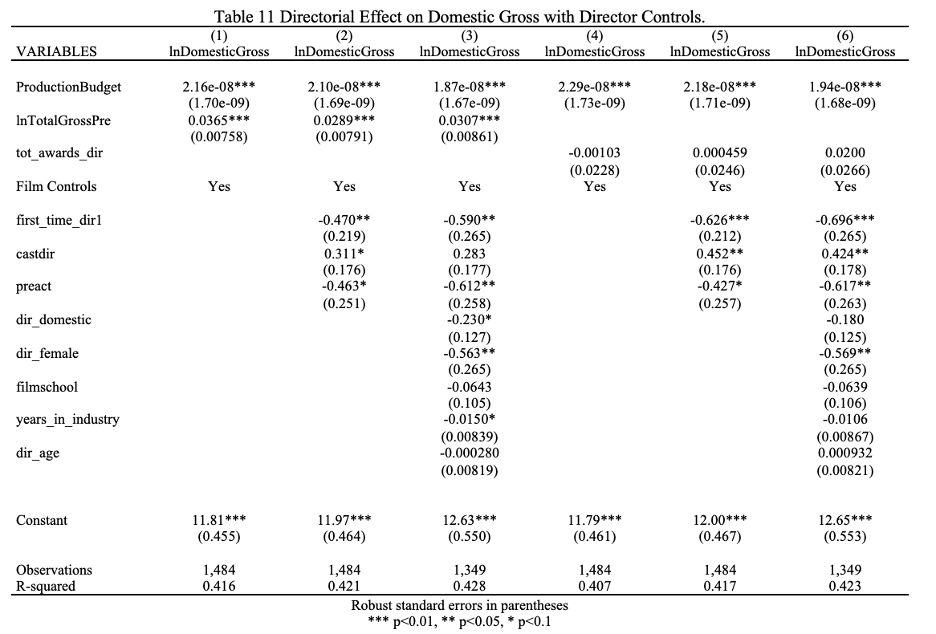
\includegraphics{./assets/thesis_table1.png}
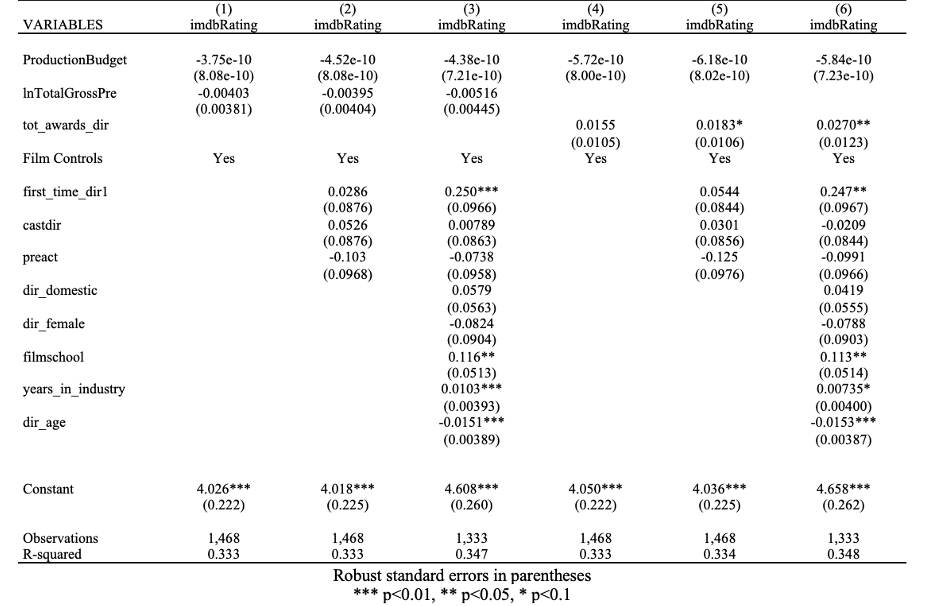
\includegraphics{./assets/thesis_table2.png}

The paper found an increase in director financial quality yielded
between a 0.0289\% and 0.0307\% increas in domestic gross and no impact
on IMDb rating. Conversely, director quality in terms of critical
acclaim yielded no significant impact on domestic gross, but betweeen
0.01803 and 0.0270 point increase in IMDb rating. The paper also
discovered a statistically significant decrease in domestic gross for
demale directors as compared to male directors.

Overall, the results were thought-provoking, however, the methodology
used was lacking in the causality department. This paper, if anything,
worked towards establishing a weak association due to it statical
analysis going only so far as a simple ordinary-least-squares regression
and controlling for confounding variables. While, the variables were
considered and included in the regression equation, they were all
treated equally as controls, thus a more complex analysis is warranted.

Furthermore, I wanted to investigate the conclusion of gender bias
further and shifted this analysis to examine actors instead of
directors.

Moving forward, the work to get to causality includes introducing
causality instead of just controlling for all covariates.

Thus, this paper will investigate the impact of gender bias in the film
industry pertaining to economic outcomes. Specifically, it will attempt
to establish a causal link between a film casting a female actress in
the leading role and the resulting box-office revenue by employing
propensity score matching.

Need to argue that there is sufficient common support between the
treatment and control groups in a dataset in order to use propensity
scores.

Data collection and preparation is discussed in Section~\ref{sec-data}.

Methodology and propensity scoring is discussed in
Section~\ref{sec-meth}

Results and anlysis are disucssed in Section~\ref{sec-results}

Conluding remarks, limitations, and future work are discussed in
Section~\ref{sec-conclusion}

\section{Data}\label{sec-data}

Data was collected from IMDb utilizing two separate APIs: OMDB and TMDB.

https://www.omdbapi.com/\\
https://www.themoviedb.org/

The datasets were merged on the movie title

Cleaning:

\begin{itemize}
\tightlist
\item
  dropped unimportant columns\\
\item
  dropped missing values and zeros\\
\item
  converted to correct data types\\
\item
  one-hot encoded categorical variables\\
\item
  Big Production Company Variable\\
\item
  Top 25 Director\\
\item
  Top 20 Writer\\
\item
  English/Other Language\\
\item
  Domestic/International
\end{itemize}

2,816 movies

61 columns

Variables:

\begin{itemize}
\tightlist
\item
  year\\
\item
  runtime\\
\item
  budget\\
\item
  Month of release\\
\item
  Day of Release**\\
\item
  Genre (Action, Adventure, Animation, Biography, Comedy, Crime,
  Documentary, Drama, Family, Fantasy, Film Noir, History, Horror,
  Music, Mystery, Romance, Sci-Fi, Sport, Thriller, War, Western w/
  Musical excluded)\\
\item
  MPAA Rating (G, GP, M, M/PG, NC-17, Not-Rated, PG, PG-13, R, TV-MA,
  Unrated w/ Accepted excluded)\\
\item
  Top Production Company\\
\item
  Top Director\\
\item
  Top Writer\\
\item
  Domestic (w/ International excluded)\\
\item
  English Language (w/ Other excluded)\\
\item
  Sentiment of Description\\
\item
  Sentiment of Tagline\\
\item
  Starpower Metric
\end{itemize}

outcomes:

\begin{itemize}
\tightlist
\item
  box office\\
\item
  imdb rating
\end{itemize}

Add in some descriptive statistics of the dataset.

\begin{longtable}[]{@{}ll@{}}
\caption{Male versus Female Director}\label{tbl-history}\tabularnewline
\toprule\noalign{}
Name & Year \\
\midrule\noalign{}
\endfirsthead
\toprule\noalign{}
Name & Year \\
\midrule\noalign{}
\endhead
\bottomrule\noalign{}
\endlastfoot
Female Leads & 488 \\
Male Leads & 2328 \\
\end{longtable}

Table~\ref{tbl-history}

\section{Methodology}\label{sec-meth}

\subsection{Sentiment Analysis of tagline and
description}\label{sentiment-analysis-of-tagline-and-description}

BERT model for sentiment analysis\\
created labels of 0/1 for tagline and movie description

\subsection{Creation of the starpower
variable}\label{creation-of-the-starpower-variable}

Collected lists of A-list and B-list actors/actresses\\
Added 2 points if one of the cast members was A-list\\
Added 1 point if one of the cast members was B-list\\
Averaged by dividing score by 3 (number of cast members)

\begin{longtable}[]{@{}
  >{\raggedright\arraybackslash}p{(\columnwidth - 6\tabcolsep) * \real{0.3014}}
  >{\raggedright\arraybackslash}p{(\columnwidth - 6\tabcolsep) * \real{0.2877}}
  >{\raggedright\arraybackslash}p{(\columnwidth - 6\tabcolsep) * \real{0.2466}}
  >{\raggedright\arraybackslash}p{(\columnwidth - 6\tabcolsep) * \real{0.1644}}@{}}
\toprule\noalign{}
\begin{minipage}[b]{\linewidth}\raggedright
actor1
\end{minipage} & \begin{minipage}[b]{\linewidth}\raggedright
actor2
\end{minipage} & \begin{minipage}[b]{\linewidth}\raggedright
actor3
\end{minipage} & \begin{minipage}[b]{\linewidth}\raggedright
starpower
\end{minipage} \\
\midrule\noalign{}
\endhead
\bottomrule\noalign{}
\endlastfoot
Mark Wahlberg & Tyrese Gibson & André 3000 & 0.666667 \\
Jamie Bell & Andy Serkis & Daniel Craig & 1.333333 \\
Ryan Reynolds & Blake Lively & Peter Sarsgaard & 0.333333 \\
Marc Singer & Tanya Roberts & Rip Torn & 0.000000 \\
Tom Hiddleston & Samuel L. Jackson & Brie Larson & 1.000000 \\
Jeremy Renner & Ed Helms & Jake Johnson & 0.000000 \\
Frankie Muniz & Amanda Bynes & Paul Giamatti & 1.000000 \\
Ben Barnes & Skandar Keynes & Georgie Henley & 0.000000 \\
Jason Bateman & Charlie Day & Jason Sudeikis & 1.000000 \\
Jack Black & Ana de la Reguera & Héctor Jiménez & 0.333333 \\
\end{longtable}

\subsection{Creation of the variable that indicates female in leading
role}\label{creation-of-the-variable-that-indicates-female-in-leading-role}

Collected list of all female actresses\\
Took the first cast member named\\
Merged and created female\_lead variable\\
1 = female lead

\begin{longtable}[]{@{}lll@{}}
\toprule\noalign{}
Title & First Actor & Female Lead \\
\midrule\noalign{}
\endhead
\bottomrule\noalign{}
\endlastfoot
The Family & Robert De Niro & 0 \\
The Shack & Sam Worthington & 0 \\
The Dead Zone & Christopher Walken & 0 \\
The Ref & Denis Leary & 0 \\
Flyboys & James Franco & 0 \\
ATL & Tip `T.I.' Harris & 0 \\
Like a Boss & Tiffany Haddish & 1 \\
Enemy Mine & Dennis Quaid & 0 \\
Proud Mary & Taraji P. Henson & 1 \\
Valmont & Colin Firth & 0 \\
\end{longtable}

\subsection{Propensity score matching}\label{propensity-score-matching}

StandardScaler Propensity scores calculated

\subsection{Robustness Checks}\label{robustness-checks}

Implemented the IMDb score as the outcome variable as a robustness
check\\
Does a female in the lead role impact the critical success of the film?

\section{Results}\label{sec-results}

\subsection{Box Office Results}\label{box-office-results}

Female-lead had higher box-office average

\subsection{IMDb Rating Results}\label{imdb-rating-results}

Female-lead had lower IMDb scores

\begin{longtable}[]{@{}lll@{}}
\toprule\noalign{}
Gender of Lead Role & Box Office & IMDb Rating \\
\midrule\noalign{}
\endhead
\bottomrule\noalign{}
\endlastfoot
Female & 62,708,871.36 & 6.329 \\
Male & 61,076,707.45 & 6.601 \\
\end{longtable}

\section{Conclusion}\label{sec-conclusion}

\subsection{Limitations:}\label{limitations}

\begin{enumerate}
\def\labelenumi{\arabic{enumi}.}
\tightlist
\item
  More data
\item
  Network Analysis
\item
  Robustness Checks with Bechdel test
\item
  Inacurracy from matching female leads \& first actor not always the
  lead
\item
  Unbalanced Dataset (is this an issue?)
\end{enumerate}

\section*{References}\label{references}
\addcontentsline{toc}{section}{References}

\vspace{1em}

\textsubscript{Source:
\href{https://ehealy19.github.io/Matching_Movies/index-preview.html}{Article
Notebook}}




\end{document}
